\section{ITK Introduction}


\centeredlargetext{white}{black}{
ITK Introduction
}

\begin{frame}
\frametitle{ITK is a Templated Library}
You will typically do:
\begin{itemize}
\item Include headers
\pause
\item Pick pixel type
\pause
\item Pick image dimension
\pause
\item Instantiate image type
\pause
\item Instantiate filter type
\pause
\item Create filters
\pause
\item Connect pipeline
\pause
\item Run pipeline
\end{itemize}
\end{frame}

{
\setbeamertemplate{navigation symbols}{}
\begin{frame}[fragile]
\frametitle{Basic Filtering}
\framesubtitle{Median Filter}
\begin{itemize}
\item Include headers\footnote{Source code in Exercises/ITKIntroduction/exercise1/BasicImageFilteringITK.cxx}
\end{itemize}
\begin{center}
\lstinputlisting[linerange={19-21}]{BasicImageFilteringITK.cxx}
\end{center}
\pause
\begin{itemize}
\item Read images from files
\item Write images from files
\item Apply a median filter in an image
\end{itemize}
\end{frame}
}

{
\setbeamertemplate{navigation symbols}{}
\begin{frame}[fragile]
\frametitle{Basic Filtering}
\framesubtitle{Median Filter}
\begin{itemize}
\item Declare pixel types and image dimension\footnote{Source code in Exercises/ITKIntroduction/exercise1/BasicImageFilteringITK.cxx}
\end{itemize}
\begin{center}
\lstinputlisting[linerange={32-35}]{BasicImageFilteringITK.cxx}
\end{center}
\pause
\begin{itemize}
\item Declare input and output image types
\end{itemize}
\begin{center}
\lstinputlisting[linerange={37-38}]{BasicImageFilteringITK.cxx}
\end{center}
\end{frame}
}

{
\setbeamertemplate{navigation symbols}{}
\begin{frame}[fragile]
\frametitle{Basic Filtering}
\framesubtitle{Median Filter}
\begin{itemize}
\item Declare the types for reader and writer\footnote{Source code in Exercises/ITKIntroduction/exercise1/BasicImageFilteringITK.cxx}
\end{itemize}
\begin{center}
\lstinputlisting[linerange={40-41}]{BasicImageFilteringITK.cxx}
\end{center}
\pause
\begin{itemize}
\item Instantiate the reader and writer objects (source and sink)
\end{itemize}
\begin{center}
\lstinputlisting[linerange={43-44}]{BasicImageFilteringITK.cxx}
\end{center}
\pause
\begin{itemize}
\item Set input and output filenames
\end{itemize}
\begin{center}
\lstinputlisting[linerange={46-47}]{BasicImageFilteringITK.cxx}
\end{center}
\end{frame}
}

{
\setbeamertemplate{navigation symbols}{}
\begin{frame}[fragile]
\frametitle{Basic Filtering}
\framesubtitle{Median Filter}
\begin{itemize}
\item Declare the Median filter type\footnote{Source code in Exercises/ITKIntroduction/exercise1/BasicImageFilteringITK.cxx}
\end{itemize}
\begin{center}
\lstinputlisting[linerange={49-50}]{BasicImageFilteringITK.cxx}
\end{center}
\pause
\begin{itemize}
\item Create the filter
\end{itemize}
\begin{center}
\lstinputlisting[linerange={51-51}]{BasicImageFilteringITK.cxx}
\end{center}
\end{frame}
}

{
\setbeamertemplate{navigation symbols}{}
\begin{frame}[fragile]
\frametitle{Basic Filtering}
\framesubtitle{Median Filter}
\begin{itemize}
\item Define the Median kernel radius (Manhattan Radius)\footnote{Source code in Exercises/ITKIntroduction/exercise1/BasicImageFilteringITK.cxx}
\end{itemize}
\begin{center}
\lstinputlisting[linerange={55-58}]{BasicImageFilteringITK.cxx}
\end{center}
\pause
\begin{itemize}
\item Connect the pipeline
\end{itemize}
\begin{center}
\lstinputlisting[linerange={60-61}]{BasicImageFilteringITK.cxx}
\end{center}
\end{frame}
}

{
\setbeamertemplate{navigation symbols}{}
\begin{frame}[fragile]
\frametitle{Basic Filtering}
\framesubtitle{Median Filter}
\begin{itemize}
\item Trigger the pipeline execution by calling Update().
\end{itemize}
\begin{center}
\lstinputlisting[linerange={63-71}]{BasicImageFilteringITK.cxx}
\end{center}
\pause
\begin{itemize}
\item ITK uses C++ exceptions for error management
\item Exceptions are typically thrown during Update() calls
\item Applications must catch the exceptions and solve them
\end{itemize}
\end{frame}
}


\begin{frame}
\frametitle{LUIS TODO}
\begin{itemize}
\item Create shortcut to build from nautilus
\item Shell script that launches gnome-terminal, cd s to binary dir and user can type "make"
\end{itemize}
\end{frame}


\begin{frame}
\frametitle{How to Configure and Build}
\framesubtitle{cmake-gui}
\begin{itemize}
\item Create a directory
\item Configure the code with CMake
\item Build (compile and link an executable)
\item Run it in example image
\end{itemize}
\end{frame}

\begin{frame}[fragile]
\frametitle{How to Configure and Build}
\framesubtitle{cmake-gui}
\begin{itemize}
\item Create a directory
\end{itemize}
\begin{verbatim}
cd ~/bin
mkdir itkexercise1
cd itkexercise1
\end{verbatim}
\end{frame}

\begin{frame}[fragile]
\frametitle{How to Configure and Build}
\framesubtitle{cmake-gui}
\begin{itemize}
\item Run ``cmake-gui''
\item Set ``Source Directory'' (where the source code is)
\item Set ``Binary Directory'' (where to build the executable)
\item Click on ``Configure''
\end{itemize}
\begin{center}
  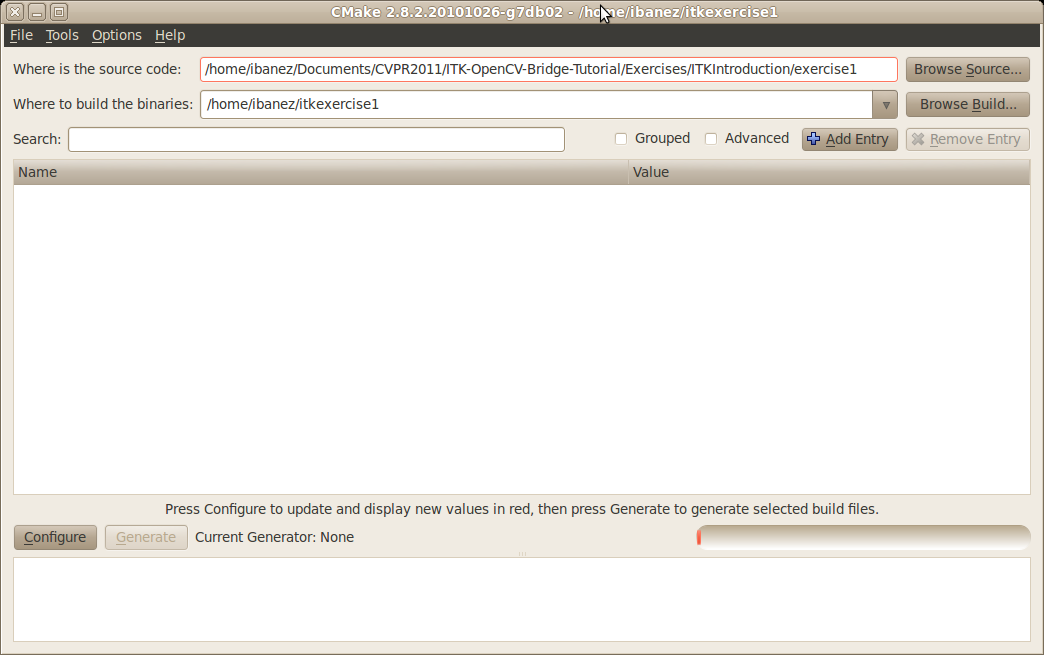
\includegraphics[width=0.5\paperwidth]{Screenshot-CMakeGUI-01.png}
\end{center}
\end{frame}

\begin{frame}[fragile]
\frametitle{How to Configure and Build}
\framesubtitle{cmake-gui}
\begin{itemize}
\item Select to generate ``Unix Makefiles''
\item Select to ``Use default native compilers''
\end{itemize}
\begin{center}
  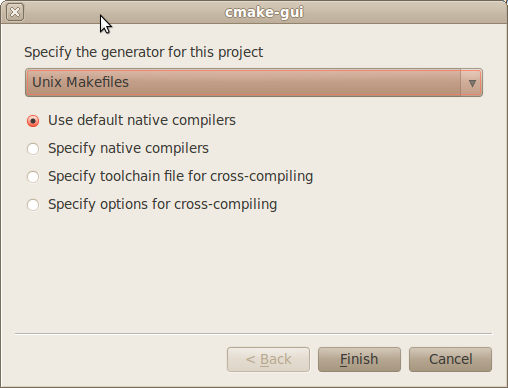
\includegraphics[width=0.5\paperwidth]{Screenshot-CMakeGUI-02.png}
\end{center}
\end{frame}

\begin{frame}[fragile]
\frametitle{How to Configure and Build}
\framesubtitle{cmake-gui}
\begin{itemize}
\item Click on ``Configure''
\item Set ``ITK\_DIR'' to /home/tutorial/bin/ITKVideo/Release
\item Click on ``Configure''
\item Click on ``Generate''
\end{itemize}
\begin{center}
  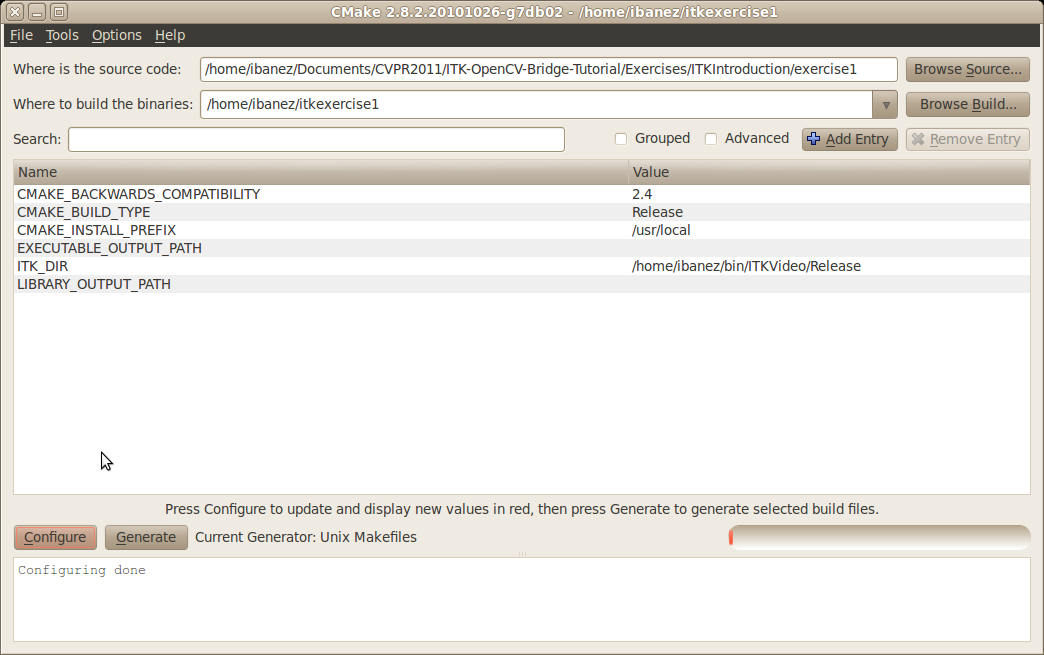
\includegraphics[width=0.5\paperwidth]{Screenshot-CMakeGUI-03.png}
\end{center}
\end{frame}

\begin{frame}[fragile]
\frametitle{How to Build}
\framesubtitle{cmake-gui}
\begin{itemize}
\item In the command line do:
\end{itemize}
\begin{verbatim}
cd  /home/tutorial/itkexercise1
make
\end{verbatim}
\end{frame}

\begin{frame}[fragile]
\frametitle{How to Run}
\framesubtitle{cmake-gui}
\begin{itemize}
\item In the command line type:
\end{itemize}
\begin{verbatim}
./BasicImageFilteringITK  ~/data/lenna.jpg  lennaMedian.png
\end{verbatim}
\end{frame}

\begin{frame}[fragile]
\frametitle{How to View the Result}
\framesubtitle{cmake-gui}
\begin{itemize}
\item In the command line type:
\end{itemize}
\begin{verbatim}
eog ~/data/lenna.jpg &
eog lennaMedian.png &
\end{verbatim}
\end{frame}


\begin{frame}
\frametitle{Basic Filtering}
\framesubtitle{Replace with Canny Filter}
\begin{center}
\lstinputlisting[linerange={21-23}]{BasicImageFilteringITK.cxx}
\end{center}
\end{frame}

